% ===================================================================
% Week 01 -- Introduction to Communication Networks (HUJI 67594)
% Sources (in materials/week01/): "1 Introduction to networking.pdf" (lecture,
% Y. Gilad) and week1.pdf (tutorial: course background + probability).
% References: Kurose & Ross, Computer Networking: A Top-Down Approach (8th ed.)
% [KR], ch. 1.3-1.4; Bertsekas & Gallager, Data Networks (2nd ed.) [BG], ch. 1, 3.3.
% Build: pdflatex -interaction=nonstopmode week01.tex  (twice)
% ===================================================================
% ===================================================================
% Preamble for the Introduction to Communication Networks weekly notes (copy of the shared
% lecture-notes preamble, kept here so this folder builds on its own).
% ===================================================================
\documentclass[11pt,a4paper]{article}

% ---------- encoding & fonts ----------
\usepackage[T1]{fontenc}
\usepackage[utf8]{inputenc}
\usepackage{lmodern}
\renewcommand{\familydefault}{\rmdefault}
\usepackage{microtype}

% ---------- layout ----------
\usepackage[a4paper,margin=2.3cm,top=2.4cm,bottom=2.6cm,headsep=0.9cm]{geometry}
\setlength{\parindent}{0pt}
\setlength{\parskip}{0.55em}
\usepackage{needspace}
\usepackage{multicol}
\usepackage[shortlabels]{enumitem}
\usepackage{array,booktabs,colortbl,tabularx}
\newcolumntype{L}[1]{>{\raggedright\arraybackslash}p{#1}}

% ---------- maths ----------
\usepackage{amsmath,amssymb,mathtools}

% ---------- colours ----------
\usepackage[dvipsnames]{xcolor}
\definecolor{paper}{HTML}{EFE9DA}
\definecolor{surface}{HTML}{FDFBF4}
\definecolor{surface2}{HTML}{F1EBDB}
\definecolor{ink}{HTML}{221C35}
\definecolor{muted}{HTML}{6E6883}
\definecolor{border}{HTML}{4B3C8E}
\definecolor{shadowcol}{HTML}{2E2552}
\definecolor{pgreen}{HTML}{1D6A3B}
\definecolor{ppink}{HTML}{D0307A}
\definecolor{pgold}{HTML}{8C5C0B}
\definecolor{pcyan}{HTML}{2B5FA8}
\pagecolor{paper}
\color{ink}

% ---------- graphics ----------
\usepackage{tikz}
\usetikzlibrary{positioning,arrows.meta,calc,shapes.geometric,shapes.misc,decorations.pathreplacing,patterns,fit,backgrounds}
\usepackage{pgfplots}
\pgfplotsset{compat=1.18}
\tikzset{
  lbl/.style={font=\footnotesize,text=ink,inner sep=1pt},
  blk/.style={draw=ink,line width=1pt,fill=surface,font=\sffamily\scriptsize\bfseries,align=center,minimum height=0.85cm,inner sep=4pt},
  arr/.style={-{Stealth},line width=1.1pt,ink},
  dot/.style={circle,fill=ink,inner sep=1.4pt},
  plbl/.style={font=\ttfamily\scriptsize,text=muted,inner sep=1pt},
  >={Stealth[length=2.6mm]}
}

% ---------- inline semantic markup ----------
\newcommand{\term}[1]{\textcolor{pgreen}{#1}}   % newly defined term
\newcommand{\key}[1]{\textcolor{pcyan}{#1}}     % key word / unit
\newcommand{\hl}[1]{\textcolor{ppink}{#1}}      % the thing to remember
\newcommand{\thd}[1]{{\color{surface}\sffamily\bfseries\footnotesize #1}} % table header cell
\newcommand{\src}[1]{{\ttfamily\scriptsize\textcolor{muted}{[#1]}}}

% ---------- boxes ----------
\usepackage[most]{tcolorbox}
\tcbset{
  notebase/.style={
    enhanced jigsaw, breakable, sharp corners,
    colback=surface, colframe=border, boxrule=1.1pt,
    left=6pt,right=6pt,top=5pt,bottom=5pt,
    before skip=1.1em, after skip=1.1em,
    shadow={1.4mm}{-1.4mm}{0mm}{fill=shadowcol},
    fonttitle=\ttfamily\scriptsize,
    attach boxed title to top left={xshift=3mm,yshift*=-2.4mm},
    boxed title style={sharp corners,boxrule=0.9pt,colframe=surface,
      left=4pt,right=4pt,top=2.5pt,bottom=2.5pt,
      shadow={0.8mm}{-0.8mm}{0mm}{fill=shadowcol}},
    parbox=false,
    before upper={\setlength{\parskip}{0.45em}},
  }
}
\newcommand{\boxtitle}[2]{\if\relax\detokenize{#2}\relax #1\else #1 \textperiodcentered\ \MakeUppercase{#2}\fi}
\newcommand{\boxtitleonly}[2]{\if\relax\detokenize{#2}\relax #1\else \MakeUppercase{#2}\fi}

\newtcolorbox{defn}[1][]{notebase,colbacktitle=pgreen,title={\boxtitle{DEF}{#1}}}
\newtcolorbox{formula}[1][]{notebase,colbacktitle=border,title={\boxtitleonly{FORMULA}{#1}}}
\newtcolorbox{intuition}[1][]{notebase,colbacktitle=ppink,title={\boxtitleonly{KEY IDEA}{#1}}}
\newtcolorbox{example}[1][]{notebase,colbacktitle=pcyan,title={\boxtitle{EXAMPLE}{#1}}}
\newtcolorbox{pitfall}[1][]{notebase,colbacktitle=pgold,title={\boxtitle{PITFALL}{#1}}}
\newtcolorbox{plainbox}{notebase}

% lists inside notes
\setlist[itemize]{label={\textcolor{pgreen}{\scriptsize$\blacksquare$}},leftmargin=1.3em,itemsep=0.25em,topsep=0.3em}
\setlist[enumerate]{label={\textcolor{pgreen}{\ttfamily\arabic*.}},leftmargin=1.6em,itemsep=0.3em,topsep=0.3em}

% ---------- headings ----------
\usepackage{titlesec}
\newcommand{\twodigit}[1]{\ifnum#1<10 0\fi\number#1}
\titleformat{\section}[display]
  {\sffamily\bfseries\fontsize{20}{24}\selectfont\color{pgold}}
  {\ttfamily\small\mdseries\color{pgreen}SECTION \twodigit{\value{section}}}
  {8pt}{}[\vspace{4pt}{\color{border}\titlerule[1.4pt]}]
\titlespacing*{\section}{0pt}{1.6em}{1.0em}
\titleformat{\subsection}
  {\ttfamily\large\color{pcyan}}{>\,\thesubsection}{0.6em}{}
\titlespacing*{\subsection}{0pt}{1.3em}{0.5em}
\titleformat{\subsubsection}
  {\sffamily\bfseries\color{border}}{\thesubsubsection}{0.6em}{}
\titlespacing*{\subsubsection}{0pt}{1.0em}{0.3em}

% ---------- running header / footer ----------
\usepackage{fancyhdr}
\newcommand{\headleft}{}
\newcommand{\headright}{}
\pagestyle{fancy}
\fancyhf{}
\renewcommand{\headrulewidth}{0pt}
\fancyhead[L]{\ttfamily\scriptsize\textcolor{muted}{\headleft}}
\fancyhead[R]{\ttfamily\scriptsize\textcolor{muted}{\headright}}
\fancyfoot[C]{\tikz{\node[draw=border,line width=1pt,fill=surface,inner sep=2.5pt,font=\sffamily\footnotesize] (p) {\thepage};
  \draw[shadowcol,line width=1.6pt] ([yshift=-2pt]p.south west)--([yshift=-2pt]p.south east);}}
\fancypagestyle{plain}{\fancyhf{}\renewcommand{\headrulewidth}{0pt}\fancyfoot[C]{\tikz{\node[draw=border,line width=1pt,fill=surface,inner sep=2.5pt,font=\sffamily\footnotesize] (p) {\thepage};
  \draw[shadowcol,line width=1.6pt] ([yshift=-2pt]p.south west)--([yshift=-2pt]p.south east);}}}

% ---------- links ----------
\usepackage[hidelinks]{hyperref}

\graphicspath{{figures/week01/}}
\renewcommand{\headleft}{67594 \textperiodcentered\ WEEK 01}
\renewcommand{\headright}{INTRODUCTION TO COMMUNICATION NETWORKS}

\newcommand{\figcap}[1]{\par\smallskip{\small\color{muted}#1}\par}
\newcommand{\tocpart}[1]{\par\smallskip{\ttfamily\scriptsize\color{pgreen}#1}\par}
\newcommand{\parttitle}[2]{%
  \clearpage
  {\ttfamily\small\color{pgreen}#1}\par\vspace{2pt}
  {\sffamily\bfseries\fontsize{26}{30}\selectfont\color{pgold}#2}\par
  \vspace{4pt}{\color{border}\rule{\linewidth}{1.8pt}}\par\vspace{0.6em}%
  \addtocontents{toc}{\protect\tocpart{#1}}}
\newcommand{\slidefig}[2]{\begin{center}\fcolorbox{border}{white}{\includegraphics[width=#1]{#2}}\end{center}}
\newcommand{\E}{\mathbb{E}}
\newcommand{\Var}{\operatorname{Var}}
\newcommand{\cmpl}[1]{\overline{#1}}

\begin{document}

% ---------------- title block ----------------
{\ttfamily\small\color{pgreen}HUJI \textperiodcentered\ 67594 \textperiodcentered\ INTRODUCTION TO COMMUNICATION NETWORKS}\par\vspace{6pt}
{\sffamily\bfseries\fontsize{30}{34}\selectfont\color{pgold}Week 01}\par\vspace{4pt}
{\sffamily\bfseries\Large\color{pgold}Introduction to Networking; Probability for Networks}\par\vspace{4pt}
{\ttfamily\small\color{pcyan}latency \textperiodcentered\ circuit switching \textperiodcentered\ packet switching \textperiodcentered\ statistical multiplexing \textperiodcentered\ Bayes \textperiodcentered\ random variables \textperiodcentered\ Poisson process}\par
\vspace{0.8em}

{\ttfamily\small\color{pgreen}CONTENTS}
\begin{multicols}{2}\footnotesize\setlength{\parskip}{0pt}
\setcounter{tocdepth}{1}
\makeatletter\@starttoc{toc}\makeatother
\end{multicols}

% =================================================================
\parttitle{PART A \textperiodcentered\ LECTURE 1}{Introduction to Networking}
% =================================================================

\section{What is a computer network?}

\begin{formula}[The ultimate goal]
A computer network exists for one job: \textbf{transmitting data between end users}.
\end{formula}

\begin{defn}[Hosts, links, nodes]
\begin{itemize}
  \item \term{End users} (also \term{hosts}, terminals, stations): the machines at the edge that \emph{produce and consume} data, such as laptops, phones and servers.
  \item \term{Links}: the physical media that carry bits between two machines, such as optical fibre, copper cable or wireless.
  \item \term{Nodes} (\term{routers}, \term{switches}): machines inside the network whose only job is to pass data along towards its destination.
\end{itemize}
``The network'' is the set of nodes and links between the hosts \src{KR 1.1}.
\end{defn}

\slidefig{0.7\linewidth}{network_birds_eye}
\figcap{The bird's-eye view (lecture slide 28): hosts (squares) attach at the edge; inside the cloud, nodes (circles) are joined by links.}

\begin{defn}[Network vs.\ distributed system]
The \term{computer network} is the infrastructure and technology that transmits data between hosts. A \term{distributed system} is the set of hosts
\emph{using} that network to do something together (a web service, a multiplayer game). \hl{The network itself produces no data}, except
control data that it needs to manage itself.
\end{defn}

\subsection{Networks of every size and every kind}

Networks range from a small home or office network to the whole Internet: in 2025 about 8.7 million users in Israel and 6.12 billion in the
world, a 73.8\% penetration rate (95\%+ in North America and northern Europe). More and more of the devices are not computers at all.

\begin{defn}[Internet of Things (IoT)]
The \term{Internet of Things} is the network of physical objects (vehicles, home appliances, locks, thermostats, insulin trackers, \dots) that
contain electronics, software, sensors and network connectivity, so that they can exchange data over the existing Internet. Each thing is uniquely identifiable.
\end{defn}

The network has to serve very different \emph{applications}, and they want different things:
\begin{defn}[Application requirements]
\begin{itemize}
  \item \textbf{Size of transfers}: ``\term{elephants}'' (huge, e.g.\ a backup) vs.\ ``\term{mice}'' (tiny, e.g.\ a web click).
  \item \textbf{Bidirectionality}: does data flow both ways (a call) or mostly one way (video streaming)?
  \item \textbf{Latency sensitivity}: does a delay hurt (a game) or not (an e-mail)?
  \item \textbf{Jitter tolerance}: \term{jitter} is the \emph{variation} in delay from packet to packet. Voice and video suffer from it.
  \item \textbf{Drop tolerance} and \textbf{reliability}: may some data be lost, or must every bit arrive?
  \item \textbf{Multicast}: should one sender reach many receivers at once?
\end{itemize}
\end{defn}

\begin{example}[Streaming video]
A video server sends a stored video to a client across the Internet. Users start leaving if the video does not start playing within \textbf{2 seconds}.
\term{DASH} (Dynamic Adaptive Streaming over HTTP) lets the client request the video chunk by chunk, each at a bitrate $r$ it chooses. The aim is good
\term{Quality of Experience} (QoE), the quality the user actually perceives. The difficulty: the video bitrate should be just below the available
network bandwidth, but on a mobile link \hl{the bandwidth changes too fast to adapt to}.
\end{example}

\begin{intuition}[The Internet ``only just'' works]
The Internet is ever more important, yet surprisingly fragile: performance is sometimes poor, it is insecure, and it is unpredictable. Applications
above it and link technologies below it innovate constantly, but the core Internet protocols in the middle (TCP/IP, BGP, DNS, OSPF, \dots)
change very slowly. Better protocols, for security, performance and evolvability, are the unsolved challenges of the field.
\end{intuition}

\section{Latency: how long does a packet take?}

\subsection{The riddle}

\begin{example}[Jerusalem $\to$ New York at the speed of light]
Distance $\approx 9{,}164$\,km, speed of light $c\approx300{,}000$\,km/s:
\[ \frac{9164\ \text{km}}{300{,}000\ \text{km/s}} \approx 0.03055\ \text{s} = 30.55\ \text{ms}. \]
No packet can ever do better: \hl{$30.55$\,ms is a hard lower bound}.
\end{example}

So how long does an Internet packet really take? It depends on:
\begin{itemize}
  \item the \textbf{route} the packet takes (rarely a straight line);
  \item the \textbf{propagation speed} of the links: in optical fibre light travels at only about $\tfrac23c$;
  \item the \textbf{transmission rate} (bandwidth, bits/s) of the links, and therefore the \textbf{size of the packet};
  \item the \textbf{number of hops} (each node adds processing delay);
  \item the \textbf{competition for bandwidth} (congestion): the packet may wait in router queues.
\end{itemize}
In practice this comes to \hl{$\ge70$\,ms one way} to New York (within Israel, $\ge10$\,ms).

\subsection{The four delays}

The lecture's list is exactly the standard decomposition of the delay at each node \src{KR 1.4.1}:

\begin{defn}[The four components of nodal delay]
\begin{itemize}
  \item \term{Processing delay} $d_{\text{proc}}$: time to read the header and decide where the packet goes (microseconds).
  \item \term{Queuing delay} $d_{\text{queue}}$: time waiting in the buffer for earlier packets to be sent. Zero on an idle link, large under congestion.
  \item \term{Transmission delay} $d_{\text{trans}} = L/R$: time to push all $L$ bits of the packet onto a link of rate $R$ bits/s.
  \item \term{Propagation delay} $d_{\text{prop}} = d/s$: time for one bit to travel the length $d$ of the link at propagation speed $s$.
\end{itemize}
\[ d_{\text{nodal}} = d_{\text{proc}} + d_{\text{queue}} + d_{\text{trans}} + d_{\text{prop}}. \]
\end{defn}

\begin{pitfall}[Transmission vs.\ propagation]
Transmission delay depends on the \emph{packet size and the link rate}, not on the distance. Propagation delay depends on the \emph{distance},
not on the packet size. A toll-booth picture: transmission = how long it takes to wave the whole convoy of cars through the booth;
propagation = how long one car takes to drive to the next booth \src{KR 1.4.1}.
\end{pitfall}

\begin{example}[Jerusalem $\to$ New York, with numbers]
\begin{itemize}
  \item Propagation in fibre, straight line: $9164/(200{,}000\text{ km/s}) \approx 45.8$\,ms. Real cables are longer than the straight line.
  \item Transmission of a 1500-byte packet ($L=12{,}000$ bits) on a 10\,Mbps link: $12{,}000/10^7 = 1.2$\,ms; on a 1\,Gbps link only $12\,\mu$s.
\end{itemize}
Over long distances, \hl{propagation dominates}; on slow links with big packets, transmission does.
\end{example}

\subsection{Why latency matters: the computer waits ``forever''}

\begin{example}[How many CPU cycles until the reply?]
A round trip to New York takes $\ge2\times70 = 140$\,ms. A PC at 3\,GHz executes
\[ 3\times10^9\ \text{cycles/s}\times0.14\ \text{s} = 420{,}000{,}000\ \text{cycles} \]
before the reply can possibly arrive. Even two directly connected machines (round trip $\approx0.2$\,ms $=200\,\mu$s) wait $600{,}000$ cycles.
\end{example}

\begin{intuition}[Consequences]
\begin{itemize}
  \item \textbf{Communication feedback is always dated}: by the time you hear about the network's state, it may have changed.
  \item \textbf{Communication is fundamentally asynchronous}: the sender cannot wait idly for each reply.
\end{itemize}
The grand challenge of the field is \emph{networking at the speed of light}.
\end{intuition}

\section{Circuit switching: the telephone network}

The first great communication network was the telephone network (Bell demonstrated the telephone in 1876, at the US Centennial Exhibition in Philadelphia).
It uses \term{circuit switching}.

\begin{defn}[Circuit switching]
Communication happens in three phases:
\begin{enumerate}
  \item \textbf{Establish}: the source sets up a \term{circuit} to the destination. Every node on the path stores information about the connection
        and \hl{reserves resources} for it. If no circuit is available, the caller gets a ``busy signal''.
  \item \textbf{Transfer}: the source sends a continual stream of data over the circuit. No destination address is needed, since the nodes already know the path.
  \item \textbf{Teardown}: when done, the source tears the circuit down and the resources are freed.
\end{enumerate}
\end{defn}

\subsection{The switch}

\slidefig{0.6\linewidth}{sharing_link}
\figcap{A node connects incoming links to outgoing links (slides 41, 51). Here the black and the orange circuits must share the same outgoing link.}

At first, a \textbf{human operator} connected the wires by hand. In 1889 Almon Brown Strowger invented the \textbf{automatic, electromechanical switch}
that did it without an operator.

\begin{pitfall}[Slide wording]
The slide says Strowger ``invents the telephone system''. He invented the \emph{automatic switching system} (the Strowger switch); the telephone system itself already existed.
\end{pitfall}

\slidefig{0.5\linewidth}{human_operator}
\figcap{Circuit switching with a human operator (slide 42): each call is a physical connection made across the switchboard.}

\subsection{Timing of circuit switching}

\slidefig{0.78\linewidth}{circuit_timing}
\figcap{Timing diagram (slide 50). Time runs downwards; each vertical line is a machine. A slanted bar is a message travelling: its vertical
thickness is the transmission delay, its slope reflects the propagation delay. Establishment needs a full round trip before any data flows; then the data streams through; then teardown.}

\textbf{Reading the diagram step by step.}
\begin{enumerate}
  \item Host 1 sends a setup request. It takes a propagation delay to reach Switch 1, which processes it and forwards it to Switch 2, and so on to Host 2.
  \item Host 2 answers. The answer travels back. Only now, \hl{one round-trip time (RTT) later}, is the circuit established.
  \item The information flows continuously along the reserved path.
  \item A teardown message frees the resources.
\end{enumerate}

\subsection{Multiplexing a link among circuits}

\begin{defn}[Multiplexing, TDM, FDM]
\term{Multiplexing} = sharing one link among several circuits.
\begin{itemize}
  \item \term{Time-division multiplexing} (TDM): each circuit gets certain \emph{time slots}, and uses the full link rate during its slot.
  \item \term{Frequency-division multiplexing} (FDM): each circuit gets certain \emph{frequencies}, and uses its band all the time.
\end{itemize}
\end{defn}

\slidefig{0.72\linewidth}{tdm_fdm}
\figcap{TDM (left) gives each colour a slice of time; FDM (right) gives each colour a slice of the frequency band (slide 52).}

\slidefig{0.72\linewidth}{tdm_frames}
\figcap{TDM in detail (slide 53): time is divided into \emph{frames}, and frames into \emph{slots}. The slot's position inside the frame tells
which conversation the data belongs to (slot 0 = blue). Sender and receiver must be synchronized.}

\begin{pitfall}[Unused slots are lost]
A slot belongs to its conversation whether or not the conversation has something to send. \hl{If a conversation does not use its circuit, that capacity is lost}.
\end{pitfall}

\begin{example}[A file over a TDM circuit \src{KR 1.3.2}]
Send a 640{,}000-bit file. Every link is a 1.536\,Mbps TDM link with 24 slots, and setting up the circuit takes 500\,ms.
\begin{enumerate}
  \item Each circuit gets $1.536\,\text{Mbps}/24 = 64$\,kbps.
  \item Transmission: $640{,}000/64{,}000 = 10$\,s.
  \item Total: $10 + 0.5 = 10.5$\,s (plus propagation).
\end{enumerate}
The transmission time does not depend on the number of links: the bits stream through the reserved path.
\end{example}

\section{Strengths and weaknesses of circuit switching}

\textbf{Strengths.} Predictable performance (known delays, no drops) and easy to reason about.

\textbf{Weakness 1: not resilient to failure.} Any failure along the path stops the transmission, and the whole transfer must restart: an ``all or nothing'' delivery model.

\textbf{Weakness 2: wastes bandwidth.}
\begin{defn}[Peak and average bandwidth]
An application has a \term{peak bandwidth} $P$ (its highest rate) and an \term{average bandwidth} $A$. Circuit switching must reserve $P$
for the application to work, so the \term{utilization} of the reservation is only $A/P$.
\end{defn}

\begin{example}[Smooth vs.\ bursty]
\begin{itemize}
  \item Voice: $P/A\approx3{:}1$, so utilization $\approx33\%$. A 2--3$\times$ waste may be acceptable.
  \item Data applications are \term{bursty}: $P/A$ of $100{:}1$ or more is common, so utilization is $\le1\%$. Reserving $100\times$ what you use on average is far too wasteful.
\end{itemize}
\end{example}

\textbf{Weakness 3: design tied to the application.} The telephone network was designed around voice. (This is part of the telephone network's design, not of circuit switching in general.)

\textbf{Weakness 4: setup time.} Every connection needs a round trip before any data flows, which badly penalizes short transfers.

\begin{example}[Setup cost for a mouse]
A 10\,kB web object over a 100\,Mbps path with a 140\,ms RTT: transmission $=80{,}000/10^8=0.8$\,ms, but setup $=140$\,ms. The setup is $175\times$ the transfer.
\end{example}

\section{How to do better: packets}

In 1964 Paul Baran (``On Distributed Communications'') proposed:
\begin{itemize}
  \item \textbf{distributed control}, with no central point of failure;
  \item transferring a message in \textbf{small blocks (packets)};
  \item \term{store-and-forward} delivery: each node receives a whole packet, stores it, then forwards it.
\end{itemize}
Leonard Kleinrock analyzed such networks and identified their key advantage: \textbf{statistical multiplexing} (\S\ref{sec:statmux}).

\subsection{A taxonomy of communication networks}

\begin{center}
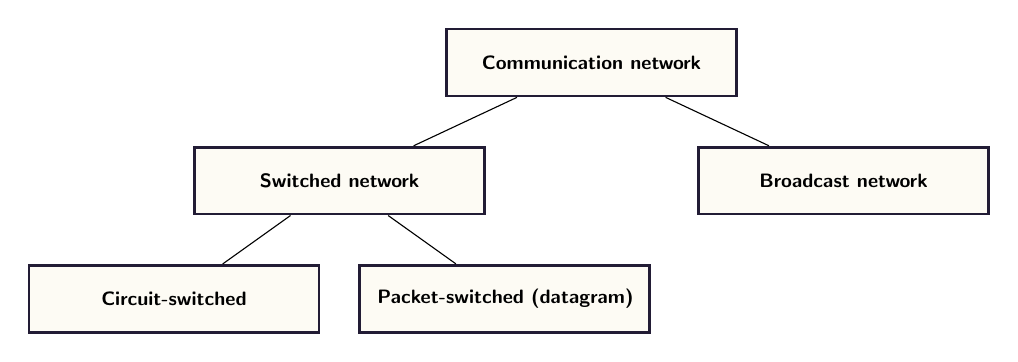
\begin{tikzpicture}[level distance=1.5cm,
  level 1/.style={sibling distance=6.4cm},
  level 2/.style={sibling distance=4.2cm},
  every node/.style={blk,text width=3.4cm}]
\node {Communication network}
  child {node {Switched network}
    child {node {Circuit-switched}}
    child {node {Packet-switched (datagram)}}}
  child {node {Broadcast network}};
\end{tikzpicture}
\figcap{Networks classified by how the nodes exchange information (slides 61--69).}
\end{center}

\begin{defn}[Broadcast network]
In a \term{broadcast network}, information transmitted by any node is \hl{received by every other node}. Usually only in LANs (local area networks),
e.g.\ WiFi, classical Ethernet, or a lecture hall. Problems:
\begin{enumerate}
  \item \textbf{limited range};
  \item \textbf{coordinating access} to the shared medium: who talks when? This is the \term{multiple access problem};
  \item \textbf{privacy}: everyone hears everything.
\end{enumerate}
\end{defn}

\section{Packet switching}

\begin{defn}[Packet / datagram]
A \term{packet} (or \term{datagram}) has two parts:
\begin{itemize}
  \item the \term{payload} (body): the data being transferred;
  \item the \term{header}: instructions to the network on how to handle the packet, above all the destination address.
\end{itemize}
Like a parcel: the contents are the payload, and the label (``To: Steve, From: Bill, Fragile'') is the header.
\end{defn}

\slidefig{0.32\linewidth}{packet}

\begin{defn}[Datagram packet switching]
\begin{itemize}
  \item \textbf{Each packet is switched independently}: each header carries the full destination address.
  \item \textbf{Nothing is reserved in advance}: no in-network resources are pre-allocated.
\end{itemize}
\end{defn}

\slidefig{0.75\linewidth}{datagram_timing}
\figcap{Timing of datagram packet switching (slide 75). No setup phase: Host 1 sends Packet 1 immediately. Each node must receive a packet
completely (store), process it, then send it on (forward). Meanwhile the next packets are already moving: a pipeline.}

\begin{formula}[Store-and-forward delay \src{KR 1.3.1}]
One packet of $L$ bits over $N$ links of rate $R$ (no queuing, ignoring propagation and processing): $\;d_{\text{end-to-end}} = N\,\dfrac{L}{R}$.
For $K$ packets back to back: $\;(N+K-1)\,\dfrac{L}{R}$.
\end{formula}

\textbf{Why $(N+K-1)$:} the first packet needs $N$ transmission times to cross the $N$ links. Each later packet arrives one transmission time after the previous one, because the links work in parallel like a pipeline.

\begin{example}[Three packets, three links]
$L=1500$ bytes $=12{,}000$ bits, $R=1.2$\,Mbps, so $L/R=10$\,ms. One packet over $N=3$ links: $30$\,ms. Three packets: $(3+3-1)\cdot10=50$\,ms,
not $90$\,ms. Compare: one 4500-byte packet would need $3\cdot30=90$\,ms. \hl{Small packets pipeline better.}
\end{example}

\slidefig{0.7\linewidth}{datagram_routes}
\figcap{Datagram switching (slide 78): packets from Host A and Host B travel through the shared nodes independently, and may even take different routes to Host D.}

\section{Bursts, buffers and queues}

\slidefig{0.7\linewidth}{bursts}
\figcap{Packets arrive in different patterns (slide 79): a smooth source (top) and a bursty one (bottom).}

\begin{intuition}[Why buffers]
Because of bursts, the \emph{transient} arrival rate is sometimes larger than the transmission rate, even if the long-term average arrival rate is smaller.
\begin{itemize}
  \item One option: \textbf{drop} the excess packets.
  \item Usually better: \textbf{buffer} them (store in a queue) until the burst ends.
\end{itemize}
But even with buffers packets are sometimes lost (a full buffer overflows), and buffers \hl{add latency} (queuing delay).
\end{intuition}

\begin{pitfall}[``Even with infinite buffers, packets are lost''?]
An infinite buffer never \emph{drops} a packet. The slide's point is that if arrivals exceed the transmission rate for long, the queue (and the delay)
grows without bound. A packet that arrives after the application has given up, or after the sender's timeout, is \emph{as good as lost}.
\end{pitfall}

\begin{defn}[Basic queueing terminology]
\begin{itemize}
  \item \term{Arrival process}: how packets arrive, with average rate $A$ and peak rate $P$.
  \item \term{Service process}: the transmission times. In networks it depends on packet size: $L/R$.
  \item $W$: the average time a packet \textbf{waits} in the queue.
  \item $L$: the average number of packets waiting in the queue (``\textbf{length} of queue'').
\end{itemize}
\end{defn}

\begin{example}[Traffic intensity \src{KR 1.4.2}]
Packets of $L_p=1000$ bits arrive on average $a=800$ per second at a 1\,Mbps link. The \term{traffic intensity} is $L_pa/R = 0.8\cdot10^6/10^6 = 0.8$.
Rule: if it exceeds $1$, the queue grows without bound. Close to $1$, the average queuing delay becomes very large even though the link is not ``full''.
\end{example}

\section{Statistical multiplexing}\label{sec:statmux}

\slidefig{0.6\linewidth}{three_flows}
\figcap{Three bursty flows and one link of a given capacity (slide 85). Each flow bursts at a different time.}

\slidefig{0.6\linewidth}{one_third_each}
\figcap{If each flow is given a fixed third of the capacity (circuit style), every burst overflows its share: frequent overloading (slide 86).
If instead all flows share the whole capacity, the bursts fit: no overloading.}

\begin{defn}[Statistical multiplexing]
\term{Statistical multiplexing} = letting many flows share a link on demand, packet by packet, instead of reserving capacity per flow. It relies
on the assumption that \hl{not all flows burst at the same time}.
\end{defn}

\begin{intuition}[Like insurance]
An insurance company collects a small premium from everyone and pays the few who have an accident. It works because not everyone crashes at once.
Statistical multiplexing has the \textbf{same failure case}: if everyone bursts at once (everyone streams the World Cup final), the shared capacity is not enough.
\end{intuition}

\subsection{How many slots per frame?}

Divide time into frames and frames into slots. Each flow generates packets every frame: at most $P$ (peak), on average $A$.
\begin{itemize}
  \item \textbf{One flow}: to never drop, allocate $P$ slots per frame. If $P\gg A$, this is very wasteful.
  \item \textbf{Many flows}: use the Law of Large Numbers.
\end{itemize}

\begin{formula}[Law of Large Numbers (Bernoulli, 1713)]
Take $N$ independent samples from \emph{any} distribution with mean $A$ (even a very variable one, from $0$ to $P$). The sum of the samples is close to
$N\times A$, and gets \hl{percentage-wise closer} as $N$ grows. So $N$ flows sharing a link need only slightly more than $A$ slots per flow per frame.
Sharing smooths out the variations.
\end{formula}

\begin{example}[How close is ``close''?]
Each flow sends $P=10$ packets in a frame with probability $0.1$ and nothing otherwise: $A=1$, standard deviation $3$.
For $N$ independent flows the total has mean $N$ and standard deviation $3\sqrt N$:
\begin{center}
\renewcommand{\arraystretch}{1.2}
\begin{tabular}{>{\columncolor{border}}c c c c c}
\thd{$N$} & \cellcolor{border}\thd{MEAN} & \cellcolor{border}\thd{STD} & \cellcolor{border}\thd{STD / MEAN} & \cellcolor{border}\thd{PEAK $N\cdot P$}\\
\rowcolor{surface} \cellcolor{border}\color{surface}10 & 10 & 9.5 & 95\% & 100\\
\rowcolor{surface2} \cellcolor{border}\color{surface}100 & 100 & 30 & 30\% & 1000\\
\rowcolor{surface} \cellcolor{border}\color{surface}1000 & 1000 & 95 & 9.5\% & 10000\\
\end{tabular}
\end{center}
With $1000$ flows, allocating mean $+$ 4 std $\approx1400$ slots covers almost every frame, versus $10{,}000$ for peak allocation.
\end{example}

\begin{pitfall}[Two fine points about the LLN]
\begin{itemize}
  \item The sum gets closer to $N\!\cdot\!A$ \emph{relatively}, not absolutely: the absolute gap grows like $\sqrt N$ ($9.5\to30\to95$ above), but the relative gap shrinks like $1/\sqrt N$.
  \item It needs the flows to be \textbf{independent}. Correlated bursts (everyone reacts to the same event) are exactly the insurance failure case.
\end{itemize}
\end{pitfall}

\begin{example}[Circuit vs.\ packet with real numbers \src{KR 1.3.2}]
Users share a 1\,Mbps link. Each user needs 100\,kbps when active and is active 10\% of the time, independently.
\begin{itemize}
  \item \textbf{Circuit switching}: reserve 100\,kbps each, so only $1\,\text{Mbps}/100\,\text{kbps}=10$ users.
  \item \textbf{Packet switching} with 35 users: the number of active users is $X\sim\text{Bin}(35,0.1)$ (Part B, \S\ref{sec:distributions}).
        The link is overloaded only if $X\ge11$: $P(X\ge11)=\sum_{k=11}^{35}\binom{35}{k}0.1^k0.9^{35-k}\approx0.0004$.
\end{itemize}
So packet switching serves \hl{3.5 times as many users} with essentially the same performance.
\end{example}

\section{Circuit switching vs.\ packet switching}

\begin{center}
\renewcommand{\arraystretch}{1.3}
\begin{tabular}{L{7.2cm} L{7.2cm}}
\rowcolor{border}\thd{CIRCUIT SWITCHING} & \thd{PACKET SWITCHING}\\
\rowcolor{surface}
\textbf{+} Guaranteed bandwidth, predictable performance (not ``best effort'').\newline
\textbf{+} Simple abstraction: a reliable channel, no lost or out-of-order packets.\newline
\textbf{+} Simple forwarding by time slot or frequency; no header to inspect.\newline
\textbf{+} Low per-packet overhead: no headers.
&
\textbf{+} Efficiency: exploits statistical multiplexing.\newline
\textbf{+} Reliability: routers keep no per-conversation state, so on a failure traffic easily moves to another path.\newline
\textbf{+} Deployability: easy for different parties to connect their networks, since nobody promises to reserve resources.\\
\rowcolor{surface2}
\textbf{--} Wasted bandwidth on bursty traffic; no statistical multiplexing gain.\newline
\textbf{--} Blocked connections: refused when resources run out, rather than ``okay'' service for everybody.\newline
\textbf{--} Per-connection state in every node, so failures are more disruptive.\newline
\textbf{--} Setup delay, which hurts small transfers.
&
\textbf{--} Must handle congestion: more complex routers (buffering, smart dropping).\newline
\textbf{--} Harder to give guarantees on delay and bandwidth.\\
\end{tabular}
\end{center}

\begin{intuition}[The verdict]
The Internet is packet-switched: efficiency, robustness and ease of deployment won over guarantees. Much of this course is about living with the
price: congestion, loss and variable delay.
\end{intuition}

% =================================================================
\parttitle{PART B \textperiodcentered\ TUTORIAL 1}{Probability for Networking}
% =================================================================

\section{Why probability?}

Most things in networks are not deterministic: whether a WiFi transmission succeeds, whether a link fails, when the next packet arrives.
Networking is largely a game of chance. We use probability mainly to
\begin{itemize}
  \item model \textbf{link and packet failure rates}, and
  \item analyse the \textbf{efficiency} of protocols and networks (as in statistical multiplexing above).
\end{itemize}

\section{Sample spaces and events}

\begin{defn}[Sample space, outcome]
The \term{sample space} $\Omega$ (\emph{merchav midgam}) is the set of all possible outcomes of an experiment. Its elements $\omega$ are the \term{outcomes}.
It can be finite or infinite, and contain numbers, letters or any symbols.
Coin: $\Omega=\{H,T\}$. Die: $\Omega=\{1,2,3,4,5,6\}$.
\end{defn}

\begin{defn}[Event; disjoint; complement]
An \term{event} (\emph{me'ora}) is a subset $A\subseteq\Omega$: a set of outcomes.
\begin{itemize}
  \item $A$ and $B$ are \term{disjoint} (\emph{zarot}) if $A\cap B=\emptyset$: they cannot both happen. Die: $A=\{1,2\}$, $B=\{4\}$.
  \item $B$ is the \term{complement} of $A$, written $\cmpl A$, if $B=\Omega\setminus A$: exactly one of them happens. With $\Omega=\{1,\dots,5\}$: $A=\{1,2,3\}$, $\cmpl A=\{4,5\}$.
\end{itemize}
\end{defn}

\section{The probability function}

\begin{defn}[Probability function]
A \term{probability function} assigns to every event $A\subseteq\Omega$ a number $P(A)$, such that
\begin{enumerate}
  \item $P(A)\in[0,1]$ for every event $A$;
  \item $P(\Omega)=1$;
  \item for disjoint events $A_1,\dots,A_n$: $\;P\big(\bigcup_iA_i\big)=\sum_iP(A_i)$ (additivity).
\end{enumerate}
\end{defn}

\begin{pitfall}[Slide notation: what is $P$ a function of?]
The slide writes $P:X\to[0,1]$ and then says ``$X$ could be $\{H,T\}$ or $\mathbb N$''. Precisely: $P$ is defined on \textbf{events}, i.e.\ on subsets of the
sample space $\Omega$, not on the elements of some set $X$. The slide's ``$X$'' plays the role of $\Omega$ (coin flip: $\Omega=\{H,T\}$; number of e-mails
per day: $\Omega=\mathbb N$), and $P$ takes subsets of it.
\end{pitfall}

\begin{example}[Fair die]
$P(\{k\})=\frac16$. Event ``even'' $=\{2,4,6\}$, three disjoint outcomes: $P=\frac16+\frac16+\frac16=\frac12$.
\end{example}

\section{Conditional probability, independence, Bayes}

\begin{defn}[Conditional probability]
The probability that $A$ happens \textbf{given that we already know} $B$ happened:
\[ P(A\mid B)=\frac{P(A\cap B)}{P(B)},\qquad P(B)>0. \]
Rearranged (the \term{multiplication rule}): $P(A\cap B)=P(A\mid B)\,P(B)$.
\end{defn}

\begin{pitfall}[Slide wording swaps the letters]
The slide describes it as ``the chance that some event $B$ will occur if we already know that $A$ had happened'', but then writes $P(A\mid B)$.
In $P(A\mid B)$ it is the other way round: $B$ is \textbf{known}, and we ask about $A$. Read the bar as ``given''.
\end{pitfall}

\begin{example}[The slide's die question]
A fair die shows an even number. How likely is it to be 2? $A=\{2\}$, $B=\{2,4,6\}$:
$P(A\mid B)=\frac{P(\{2\})}{P(\{2,4,6\})}=\frac{1/6}{1/2}=\frac13$.
\end{example}

\begin{defn}[Independence]
$A$ and $B$ are \term{independent} if $P(A\cap B)=P(A)\,P(B)$. When $P(B)>0$ this is the same as $P(A\mid B)=P(A)$: knowing $B$ tells nothing about $A$.
\end{defn}

\begin{pitfall}[Disjoint $\neq$ independent]
Disjoint events with positive probabilities are never independent: if $A\cap B=\emptyset$ then $P(A\cap B)=0\neq P(A)P(B)$. Knowing that $B$ happened tells you for certain that $A$ did \emph{not}.
\end{pitfall}

\begin{formula}[Union bound]
$P(A\cup B)\le P(A)+P(B)$, with equality when $A,B$ are disjoint. (In general $P(A\cup B)=P(A)+P(B)-P(A\cap B)$.)
\end{formula}

\begin{formula}[Bayes' theorem]
\[ P(A\mid B)=\frac{P(B\mid A)\,P(A)}{P(B)}. \]
Proof: both $P(A\mid B)P(B)$ and $P(B\mid A)P(A)$ equal $P(A\cap B)$.
\end{formula}

\begin{formula}[Law of total probability]
If $B_1,\dots,B_n$ are disjoint and $\bigcup_iB_i=\Omega$ (a \term{partition}), then for any event $D$:
\[ P(D)=\sum_{i=1}^nP(D\mid B_i)\,P(B_i). \]
\end{formula}

\begin{formula}[Complete Bayes' theorem]
For a partition $B_1,\dots,B_n$ and any $j$:
\[ P(B_j\mid D)=\frac{P(D\mid B_j)\,P(B_j)}{\sum_{i=1}^nP(D\mid B_i)\,P(B_i)}. \]
\end{formula}

\begin{pitfall}[The slide's version]
The slide writes $P(A\mid D)=\frac{P(D\mid A)P(A)}{\sum_iP(D\mid B_i)P(B_i)}$. This is correct only when $A$ is \emph{one of the} $B_j$.
The denominator is just $P(D)$ written with the law of total probability.
\end{pitfall}

\section{Worked example: good and bad packets}

A network has two types of packets:
\begin{itemize}
  \item \textbf{good} packets survive at least $T$ seconds with probability $e^{-T}$;
  \item \textbf{bad} packets survive at least $T$ seconds with probability $e^{-1000T}$.
\end{itemize}
A created packet is good with probability $p$.

\begin{example}[Question 1: survival probability]
One packet is created at $T=0$. What is the probability it still exists at $T=t$?

\textbf{Solution.} Events: $A$ = ``the packet survived $t$ seconds'', $B$ = ``it is good''. $B$ and $\cmpl B$ partition $\Omega$, so by total probability:
\[ P(A)=P(A\mid B)P(B)+P(A\mid\cmpl B)P(\cmpl B)=e^{-t}p+e^{-1000t}(1-p). \]
\end{example}

\begin{example}[Question 2: was it a good packet?]
The packet survived $t$ seconds. What is the probability it is good?

\textbf{Solution.} Bayes:
\[ P(B\mid A)=\frac{P(A\mid B)P(B)}{P(A)}=\frac{e^{-t}p}{e^{-t}p+e^{-1000t}(1-p)}. \]
\end{example}

\begin{example}[With numbers, $p=0.5$]
\begin{center}
\renewcommand{\arraystretch}{1.2}
\begin{tabular}{>{\columncolor{border}}c c c}
\thd{$t$ (s)} & \cellcolor{border}\thd{$P(A)$ survived} & \cellcolor{border}\thd{$P(B\mid A)$ good, given survived}\\
\rowcolor{surface} \cellcolor{border}\color{surface}0 & 1 & 0.5\\
\rowcolor{surface2} \cellcolor{border}\color{surface}0.001 & 0.683 & 0.731\\
\rowcolor{surface} \cellcolor{border}\color{surface}0.005 & 0.501 & 0.993\\
\rowcolor{surface2} \cellcolor{border}\color{surface}0.01 & 0.495 & 0.99995\\
\end{tabular}
\end{center}
Bad packets die within milliseconds. So \hl{surviving even 5\,ms is almost proof that the packet is good}: survival is evidence, and Bayes turns it into a probability.
\end{example}

\section{Random variables}

\begin{defn}[Random variable]
A \term{random variable} (\emph{mishtane mikri}) is a function $X:\Omega\to\mathbb R$: it attaches a number to each outcome.
It is \term{discrete} if it takes countably many values (a coin, a count), and \term{continuous} if it takes values in an interval (a time).
\end{defn}

\begin{defn}[Indicator]
The \term{indicator} of heads on a coin: $I_H(\omega)=1$ if $\omega=H$ and $0$ if $\omega=T$. In general $I_A(\omega)=1$ if $\omega\in A$, else $0$, and $\E[I_A]=P(A)$.
\end{defn}

\begin{formula}[Distribution of a discrete random variable]
\[ P(X=x)=P\big(\{\omega\in\Omega: X(\omega)=x\}\big). \]
Fair coin: $P(I_H=1)=P(\{H\})=\frac12$.
\end{formula}

\begin{pitfall}[Two notation slips on the slide]
\begin{itemize}
  \item The slide writes $\{\omega\subseteq\Omega:\dots\}$. Outcomes are \emph{elements} of $\Omega$: it should be $\omega\in\Omega$.
  \item For a coin with bias $b$, the slide writes $I_X = b$ if $\omega=H$ and $1-b$ if $\omega=T$. That mixes the random variable with its probabilities.
        The random variable is still $X(H)=1$, $X(T)=0$; the bias changes the \emph{probabilities}: $P(X=1)=b$, $P(X=0)=1-b$.
\end{itemize}
\end{pitfall}

\section{Expected value and variance}

\begin{defn}[Expected value]
The \term{expected value} (\emph{tochelet}) is the probability-weighted average of the values:
\[ \E(X)=\sum_ix_i\,P(X=x_i). \]
It is the long-run average of many independent repetitions of the experiment.
\end{defn}

\begin{formula}[Linearity and variance]
\[ \E\Big(\sum_ia_iX_i\Big)=\sum_ia_i\,\E(X_i)\qquad\text{(always, even for dependent }X_i), \]
\[ \Var(X)=\E\big((X-\E X)^2\big)=\E[X^2]-(\E X)^2. \]
\end{formula}

\begin{example}[A fair die]
$\E X=\frac{1+\dots+6}{6}=3.5$. $\E[X^2]=\frac{1+4+9+16+25+36}{6}=\frac{91}6\approx15.17$. $\Var X=15.17-12.25\approx2.92$.
\end{example}

\subsection{The four discrete distributions}\label{sec:distributions}

\begin{center}
\renewcommand{\arraystretch}{1.35}
\small
\begin{tabular}{>{\columncolor{border}}l L{3cm} L{3.1cm} L{3.1cm} L{3cm}}
 & \cellcolor{border}\thd{BERNOULLI} & \cellcolor{border}\thd{BINOMIAL} & \cellcolor{border}\thd{GEOMETRIC} & \cellcolor{border}\thd{POISSON}\\
\rowcolor{surface}\cellcolor{border}\color{surface}Story & one experiment: success or failure & successes in $n$ independent Bernoulli trials & number of independent trials until the first success & number of events in a period of time\\
\rowcolor{surface2}\cellcolor{border}\color{surface}PMF & $P(1)=p$, $P(0)=1-p$ & $\binom nkp^k(1-p)^{n-k}$ & $(1-p)^{k-1}p$, $k\ge1$ & $\dfrac{\lambda^k}{k!}e^{-\lambda}$\\
\rowcolor{surface}\cellcolor{border}\color{surface}Notation & $\text{Ber}(p)$ & $\text{Bin}(n,p)$ & $\text{Geo}(p)$ & $\text{Pois}(\lambda)$\\
\rowcolor{surface2}\cellcolor{border}\color{surface}$\E X$ & $p$ & $np$ & $1/p$ & $\lambda$\\
\rowcolor{surface}\cellcolor{border}\color{surface}$\Var X$ & $p(1-p)$ & $np(1-p)$ & $(1-p)/p^2$ & $\lambda$\\
\end{tabular}
\end{center}

\begin{example}[Why the geometric mean is $1/p$]
If each try succeeds with probability $p=0.2$, then on average one try in five succeeds, so you wait $1/0.2=5$ tries. Check the first terms:
$P(X=1)=0.2$, $P(X=2)=0.8\cdot0.2=0.16$, $P(X=3)=0.64\cdot0.2=0.128$: decreasing by the factor $0.8$ each step.
\end{example}

\section{Worked example: a chain of links}

\begin{center}
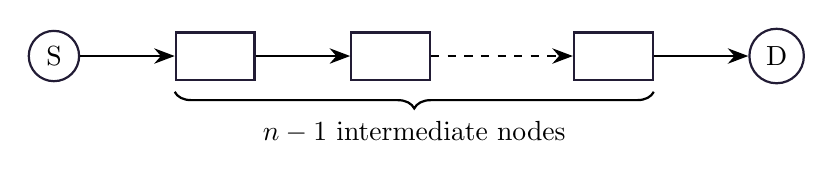
\begin{tikzpicture}[node distance=1.2cm]
  \node[circle,draw=ink,thick] (S) {S};
  \node[draw=ink,thick,minimum width=1cm,minimum height=0.6cm,right=of S] (a) {};
  \node[draw=ink,thick,minimum width=1cm,minimum height=0.6cm,right=of a] (b) {};
  \node[draw=ink,thick,minimum width=1cm,minimum height=0.6cm,right=1.8cm of b] (c) {};
  \node[circle,draw=ink,thick,right=of c] (D) {D};
  \draw[->,thick] (S)--(a); \draw[->,thick] (a)--(b); \draw[->,thick,dashed] (b)--(c); \draw[->,thick] (c)--(D);
  \draw[decorate,decoration={brace,mirror,amplitude=6pt},thick] ([yshift=-4pt]a.south west)--([yshift=-4pt]c.south east) node[midway,below=7pt]{$n-1$ intermediate nodes};
\end{tikzpicture}
\figcap{Node S sends to node D over a chain of $n$ links ($n-1$ intermediate nodes). Each link fails independently with probability $p$.}
\end{center}

\begin{example}[Question 1: does D get the message?]
\textbf{Solution.} D gets it iff \emph{no} link fails. Each link succeeds with probability $1-p$, and the links are \textbf{independent}, so the probability that all $n$ succeed is the product:
\[ P(\text{success})=(1-p)^n. \]
Numbers: $n=10$, $p=0.01$: $(0.99)^{10}\approx0.904$. Even with 99\%-reliable links, a 10-hop path fails almost 10\% of the time.
\end{example}

\begin{pitfall}[The slide says ``disjoint''; it means ``independent'']
The slide justifies the product with ``each event of a link failing is \emph{disjoint}, so the probability of the \emph{union} is the multiplication''.
That is wrong twice: we multiply because the link events are \textbf{independent}, and the product gives the probability of the \textbf{intersection}
(all links succeed), not of a union. For disjoint events we would \emph{add} probabilities of a union.
\end{pitfall}

\begin{example}[Question 2: retransmit end to end until success]
If the message is lost, S sends it again, until D gets it. Expected number of transmissions?

\textbf{Solution.} Each attempt succeeds independently with probability $q=(1-p)^n$. The number of attempts is $X\sim\text{Geo}\big((1-p)^n\big)$, so
\[ \E(X)=\frac{1}{(1-p)^n}. \]
Numbers: $n=10$, $p=0.01$: $1/0.904\approx1.11$ attempts. With $p=0.1$: $1/0.9^{10}\approx2.87$.
\end{example}

\begin{example}[Question 3: hop-by-hop retransmission]
Now every node keeps resending to its next hop until it gets through, except S, which sends only once. Probability that D gets the message?

\textbf{Solution.} Every hop after the first eventually succeeds (with probability 1). Only the first link matters: $P=1-p$.
\end{example}

\begin{example}[Question 4: sends per node]
Expected number of transmissions by one (retransmitting) node until its hop succeeds?

\textbf{Solution.} $X\sim\text{Geo}(1-p)$, so $\E(X)=\dfrac1{1-p}$. With $p=0.1$: $\approx1.11$ per hop.
\end{example}

\begin{intuition}[End-to-end vs.\ hop-by-hop]
With $p=0.1$ and $n=10$: end-to-end retransmission needs on average $2.87$ attempts. An attempt uses link $k$ only if links $1,\dots,k-1$ worked,
so it costs on average $\sum_{k=1}^{10}0.9^{k-1}=\frac{1-0.9^{10}}{0.1}\approx6.5$ link transmissions; in total $\approx2.87\times6.5\approx18.7$.
Hop-by-hop needs only $10\times1.11\approx11.1$ link transmissions. Where to retransmit (at each link or end to end) is a design choice we will meet again.
\end{intuition}

\section{Continuous random variables}

For a continuous quantity such as a time:
\begin{itemize}
  \item every single value has probability $0$, so we only ask about intervals, $P(a\le X\le b)$;
  \item probabilities are \textbf{areas} under a \term{density} $f(x)$.
\end{itemize}
\begin{formula}[Density]
\[ P(a\le X\le b)=\int_a^bf(x)\,dx,\qquad\int_{-\infty}^{\infty}f(x)\,dx=1, \]
\[ \E(X)=\int_{-\infty}^{\infty}x\,f(x)\,dx,\qquad \Var(X)=\int_{-\infty}^{\infty}(x-\E X)^2f(x)\,dx. \]
\end{formula}

\begin{center}
\renewcommand{\arraystretch}{1.4}
\begin{tabular}{>{\columncolor{border}}l L{3.6cm} L{3.6cm} L{4.2cm}}
 & \cellcolor{border}\thd{UNIFORM} & \cellcolor{border}\thd{EXPONENTIAL} & \cellcolor{border}\thd{GAUSSIAN (NORMAL)}\\
\rowcolor{surface}\cellcolor{border}\color{surface}Notation & $\text{Uni}(a,b)$ & $\text{Exp}(\lambda)$ & $N(\mu,\sigma^2)$\\
\rowcolor{surface2}\cellcolor{border}\color{surface}Density & $\frac1{b-a}$ on $[a,b]$, else $0$ & $\lambda e^{-\lambda x}$ for $x\ge0$, else $0$ & $\frac{1}{\sqrt{2\pi}\sigma}e^{-(x-\mu)^2/2\sigma^2}$\\
\rowcolor{surface}\cellcolor{border}\color{surface}$\E X$ & $\frac{a+b}2$ & $\frac1\lambda$ & $\mu$\\
\rowcolor{surface2}\cellcolor{border}\color{surface}$\Var X$ & $\frac{(b-a)^2}{12}$ & $\frac1{\lambda^2}$ & $\sigma^2$\\
\end{tabular}
\end{center}

\begin{pitfall}[Gaussian variance]
The slide's table gives $\Var(X)=\sigma$ for the Gaussian. The variance is \textbf{$\sigma^2$}; $\sigma$ is the standard deviation. Also note the
convention: here $N(\mu,\sigma^2)$ lists the variance (the slide writes $N(\mu,\sigma)$, listing the standard deviation). Check which one a source uses.
\end{pitfall}

\begin{example}[Exponential with numbers]
Time to the next packet $X\sim\text{Exp}(\lambda=2/\text{s})$: mean $0.5$\,s. $P(X>1)=e^{-2}\approx0.135$; $P(X\le0.25)=1-e^{-0.5}\approx0.39$.
\end{example}

\section{Memorylessness}

\begin{defn}[Memoryless]
A random variable $X$ is \term{memoryless} (\emph{chosser zikaron}) if for all $s,t\ge0$
\[ P(X>s+t\mid X>t)=P(X>s). \]
Having already waited $t$ does not change how much longer you have to wait. The \textbf{exponential} (continuous) and \textbf{geometric} (discrete, integer $s,t$) distributions are memoryless.
\end{defn}

\textbf{Proof for the exponential.} $P(X>x)=e^{-\lambda x}$. Then
\[ P(X>s+t\mid X>t)=\frac{P(X>s+t)}{P(X>t)}=\frac{e^{-\lambda(s+t)}}{e^{-\lambda t}}=e^{-\lambda s}=P(X>s). \]
(The intersection $\{X>s+t\}\cap\{X>t\}$ is just $\{X>s+t\}$.)

\begin{example}[Customers]
Customers arrive with exponential gaps. The time from the 9th customer's arrival to the next arrival has the same distribution as the time from opening to the first customer.
\hl{Where you are in time does not matter.}
\end{example}

\section{Random processes and the Poisson process}

\begin{defn}[Random (stochastic) process]
A \term{random process} models a system that evolves randomly in time: a family of random variables indexed by time. Observing it twice from the same start
may give different results. In networks, the times packets enter and leave a router are not predetermined, so we model them as a random process
(and also traffic demand and available resources).
\end{defn}

\begin{example}[Bernoulli process]
A sequence of i.i.d.\ Bernoulli($p$) trials. The number of successes after $n$ steps is $\text{Bin}(n,p)$.
(\term{i.i.d.} = independent and identically distributed.)
\end{example}

\begin{defn}[Inter-arrival times and arrival epochs]
Let $X_i>0$ be the time between the $(i-1)$-th and the $i$-th arrival (the \term{inter-arrival time}). The \term{arrival epochs} are
\[ S_1=X_1,\quad S_2=S_1+X_2,\quad\dots,\quad S_i=S_{i-1}+X_i: \]
the moment the $i$-th event happens.
\end{defn}

\begin{pitfall}[What $X_i$ measures]
The slide calls $X_i$ ``the time it takes the $i$-th packet to arrive''. It is the time \emph{since the previous arrival}, not since time $0$.
The time since $0$ is the epoch $S_i$.
\end{pitfall}

\begin{center}
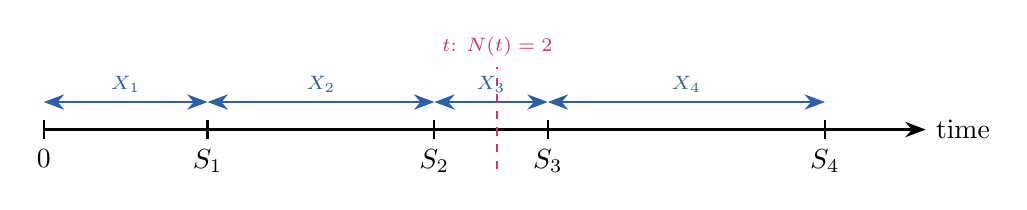
\begin{tikzpicture}[xscale=1.6]
  \draw[->,thick] (0,0)--(7,0) node[right]{time};
  \foreach \x/\l in {0/0,1.3/S_1,3.1/S_2,4.0/S_3,6.2/S_4}{\draw[thick] (\x,0.12)--(\x,-0.12) node[below]{$\l$};}
  \draw[<->,pcyan] (0,0.35)--(1.3,0.35) node[midway,above,font=\scriptsize]{$X_1$};
  \draw[<->,pcyan] (1.3,0.35)--(3.1,0.35) node[midway,above,font=\scriptsize]{$X_2$};
  \draw[<->,pcyan] (3.1,0.35)--(4.0,0.35) node[midway,above,font=\scriptsize]{$X_3$};
  \draw[<->,pcyan] (4.0,0.35)--(6.2,0.35) node[midway,above,font=\scriptsize]{$X_4$};
  \draw[ppink,thick,dashed] (3.6,-0.5)--(3.6,0.8) node[above,font=\scriptsize]{$t$: $N(t)=2$};
\end{tikzpicture}
\figcap{Inter-arrival times $X_i$, arrival epochs $S_i$, and the count $N(t)$: $N(t)=n$ exactly when $S_n\le t<S_{n+1}$.}
\end{center}

\begin{defn}[Counting process]
A \term{counting process} $\{N_t\mid t\ge0\}$ counts the arrivals up to time $t$:
\begin{itemize}
  \item $N_0=0$ and $N_t\ge0$ is an integer;
  \item monotone: $s\le t\Rightarrow N_s\le N_t$; and $N_t-N_s$ is the number of events in $(s,t]$.
\end{itemize}
The slide's picture: throwing frisbees, ``how many have I caught so far?''
\end{defn}

\begin{defn}[Poisson process]
A \term{Poisson process} with rate $\lambda$ is a counting process with
\begin{enumerate}
  \item \textbf{independent increments}: counts in disjoint intervals are independent;
  \item \textbf{stationary increments}: the count in \emph{any} interval of length $t$ is $\text{Pois}(\lambda t)$, so it depends only on the length, not on where the interval is. In particular $\E[N_t]=\lambda t$;
  \item \textbf{no bunching}: the probability of more than one arrival in a tiny interval is negligible.
\end{enumerate}
\end{defn}

\begin{example}[Is boarding a bus a Poisson process?]
\textbf{No.} Passengers board in groups at stops (bunching, violating 3), and more board at rush hour (the rate depends on the time, violating 2).
\end{example}

\begin{formula}[Inter-arrival times]
In a Poisson process with rate $\lambda$, the inter-arrival times $X_i$ are \textbf{i.i.d.\ $\text{Exp}(\lambda)$}. (This is where memorylessness comes from:
at any moment, the wait for the next arrival is $\text{Exp}(\lambda)$, however long you have already waited \src{BG 3.3}.)
\end{formula}

\begin{example}[Exactly one packet in an interval]
Packets are transmitted as a Poisson process: in an interval of length $T$ the count is $X\sim\text{Pois}(gT)$. Probability of exactly one?
\[ P(X=1)=\frac{(gT)^1}{1!}e^{-gT}=gT\,e^{-gT}. \]
Numbers: $gT=0.5\Rightarrow0.303$; $gT=1\Rightarrow0.368$; $gT=2\Rightarrow0.271$. It is largest at $gT=1$, where it equals $1/e\approx0.37$.
(This exact formula reappears in the analysis of the ALOHA random-access protocol, where ``exactly one'' means ``no collision'' \src{KR 6.3.2}.)
\end{example}

% =================================================================
\parttitle{WEEK 01}{Practice Problems and Summary}
% =================================================================

\section{Practice problems with full solutions}

\begin{example}[P1: Delays]
A 1000-byte packet goes over one 2000\,km fibre link ($s=2\times10^8$\,m/s) at 8\,Mbps. Find $d_{\text{trans}}$ and $d_{\text{prop}}$.

\textbf{Solution.} $d_{\text{trans}}=8000/(8\times10^6)=1$\,ms. $d_{\text{prop}}=2\times10^6/(2\times10^8)=10$\,ms. Propagation dominates.
\end{example}

\begin{example}[P2: Store and forward]
5 packets of 1\,ms transmission time each cross 4 links. When does the last one arrive (no queuing, no propagation)?

\textbf{Solution.} $(N+K-1)L/R=(4+5-1)\cdot1=8$\,ms.
\end{example}

\begin{example}[P3: Circuit utilization]
A video call has peak 6\,Mbps and average 2\,Mbps. What fraction of a circuit reservation is used? How many such calls fit on a 60\,Mbps circuit-switched link?

\textbf{Solution.} $A/P=2/6=33\%$. Reserving the peak: $60/6=10$ calls (on average using only 20\,Mbps).
\end{example}

\begin{example}[P4: Bayes on links]
A link is ``bad'' with probability 0.2. A bad link drops a packet with probability 0.5, a good one with probability 0.01. A packet was dropped. Probability the link is bad?

\textbf{Solution.} $P(\text{drop})=0.5\cdot0.2+0.01\cdot0.8=0.108$. $P(\text{bad}\mid\text{drop})=0.1/0.108\approx0.926$.
\end{example}

\begin{example}[P5: Geometric]
Each transmission succeeds with probability 0.75. Expected number of transmissions? Probability that more than 2 are needed?

\textbf{Solution.} $\E X=1/0.75\approx1.33$. $P(X>2)=P(\text{first two fail})=0.25^2=0.0625$.
\end{example}

\begin{example}[P6: Poisson]
Packets arrive at rate $\lambda=3$ per ms. Probability of no arrival in 1\,ms? Expected wait for the next packet?

\textbf{Solution.} $P(N=0)=e^{-3}\approx0.05$. Inter-arrival $\sim\text{Exp}(3)$, so the mean wait is $1/3$\,ms, no matter how long you have already waited.
\end{example}

\section{Cheat sheet}

\begin{formula}[Week 01 on one page]
\begin{itemize}
  \item Network = hosts (edge) + nodes (routers/switches) + links. It moves data; it produces none (except control).
  \item Delay: $d_{\text{proc}}+d_{\text{queue}}+L/R+d/s$. Light: Jerusalem--NY $\ge30.55$\,ms (vacuum); in practice $\ge70$\,ms; RTT $\ge140$\,ms $=4.2\times10^8$ cycles at 3\,GHz.
  \item \textbf{Circuit switching}: establish (1 RTT) / transfer / teardown; resources reserved; TDM or FDM; unused capacity lost. Utilization $A/P$.
  \item \textbf{Packet switching}: header + payload; each packet routed independently; nothing reserved; store-and-forward $N L/R$; $K$ packets $(N+K-1)L/R$.
  \item Bursts $\Rightarrow$ buffers $\Rightarrow$ queuing delay and possible loss. $W$ = mean wait, $L$ = mean queue length. Traffic intensity $La/R<1$.
  \item \textbf{Statistical multiplexing}: share on demand; LLN $\Rightarrow$ $N$ independent flows need $\approx NA$ (relative spread $\sim1/\sqrt N$). Fails when bursts are correlated.
  \item $P(A\mid B)=P(A\cap B)/P(B)$; independent: $P(A\cap B)=P(A)P(B)$; disjoint $\neq$ independent; total probability; Bayes.
  \item Ber($p$): $p$, $p(1-p)$. Bin($n,p$): $np$, $np(1-p)$. Geo($p$): $1/p$, $(1-p)/p^2$. Pois($\lambda$): $\lambda$, $\lambda$.
  \item Uni($a,b$): $\frac{a+b}2$, $\frac{(b-a)^2}{12}$. Exp($\lambda$): $\frac1\lambda$, $\frac1{\lambda^2}$. $N(\mu,\sigma^2)$: $\mu$, $\sigma^2$.
  \item Memoryless: $P(X>s+t\mid X>t)=P(X>s)$: exponential and geometric.
  \item Poisson process: independent + stationary increments, no bunching; $N_t\sim\text{Pois}(\lambda t)$; gaps i.i.d.\ Exp($\lambda$).
\end{itemize}
\end{formula}

\end{document}
